\documentclass[12pt]{article}
	\usepackage{mgates-letter}
	\definecolor{dark_blue} {rgb}{0., 0., 0.65}
	
	\usepackage{textcomp}
	\usepackage{mathrsfs}  % mathscr font
	\usepackage{boxedminipage}
	\usepackage{rotating}
	\usepackage{svg}
	%\usepackage{natbib}
	\usepackage[colorlinks, filecolor=dark_blue, urlcolor=dark_blue, linkcolor=black, citecolor=black]{hyperref}
\begin{document}

\title{Towards a democratized landscape for the development of Collective Adaptive Systems}
\author{Leonardo Micelli}
\date{\today}
\maketitle

\noindent


% ----------------------------------------
\newpage
\setcounter{tocdepth}{2}

% set these after the TOC
\setlength{\parindent}{0em}
\setlength{\parskip}{1em}

% ----------------------------------------
\section{State of the Art}
\paragraph{\textbf{Collective Adaptive Systems}} Collective Adaptive Systems are composed of multiple autonomous, interacting entities that operate in open-ended environments. 
They are capable of self-organization, self-adaptation, and emergent coordination—properties crucial for systems that must continue to function under continuous change and uncertainty.
In CAS, global behavior arises not from centralized planning but from local interactions among components, much like natural collectives such as ant colonies or bird flocks.

\paragraph{\textbf{Macroprogramming}} Macroprogramming\cite{10.1145/3579353} is a paradigm that expresses the macroscopic behavior of a collective system using a single program, with the aim of
capturing the global behavior of the system while abstracting away the complexities of individual components.

\paragraph{\textbf{Aggregate Computing and Field Calculus}} AC\cite{beal2016aggregate} is a macroprogramming approach that aims to ease the engineering of CAS by shifting the
focus from the individual device perspective to large aggregations of devices. It does so by exploiting the concepts of computational fields and FC.
Within the FC, a computational field is a function mapping every computational device in a network, represented by a dynamic and reflexive neighboring
relationship between devices, to a computational object. The main goal is to express the aggregate system behavior
through a functional composition of fundamental operators that manipulate (evolve, combine, restrict)
computational fields. A key concept of Field Calculus is that these aggregate-level specifications can
also be interpreted as a local set of rules that define the iterative asynchronous execution of computation rounds.

TODO: si potrebbe riformulare spiegando più nel dettaglio event structures e i self-stabilizing operators???

\paragraph{\textbf{Aggregate Computing Incarnations}} Research on AC has led to the development of several incarnations, each of them tackling various research challenges of AC.
\textit{Scafi}\cite{casadei2016towards} is one of the most actively researched and maintained implementations of
AC. It is hosted in the Scala language, a powerful and expressive JVM-based language. The main advantage of Scafi is its ability to provide a
more high-level platform to support agile prototyping for research. \textit{Collektive} is a Kotlin-based implementation of AC that provides an extension of FC via the eXchange Calculus (XC) \cite{audrito2024exchange}.
It provides an expressive DSL and it is natively multi-platform, enabling AC on a wider range of targets.
\textit{FCCP}\cite{audrito2024fcpp} is a C++ library that implements FC. It has been designed and developed to bring the AC paradigm to
resource-constrained devices that cannot support the JVM. It does so by providing an extensible C++ library and a performance-oriented simulator that allows
the developer to speed up the development process of aggregate programs.

\paragraph{\textbf{Swarm Robotics}} Swarm robotics is an approach to collective robotics that draws inspiration from the self-organized behavior of social animals \cite{brambilla2013swarm}. The goal is to design robust, flexible and scalable 
collective behaviors for large number of robots through simple rules and local interactions. There are two main methods for designing such systems: \textit{automatic design}, which employs methods derived from
evolutionary robotics and multi-robot reinforcement learning, and \textit{behavior-based design}, which involves the design and implementation of algorithms that can be executed by the robots. This design approach is often realized
in a bottom-up fashion, starting from the individual behavior of the robots. Conversely, the top-down approach is based on the idea of expressing the desired behavior of the swarm by expressing a set of instruction at the collective level.
Another important distinction is between \textit{centralized} and \textit{decentralized} approaches. Centralized approaches rely on a central entity that coordinates the behavior of the swarm, while decentralized approaches rely on local interactions between the robots to achieve the desired behavior.
Decentralized approaches, in particular, offer several interesting properties such as robustness, fault tolerance and scalability, while centralized approaches are often more efficient and easier to implement.
The field of swarm robotics has found several applications in various domains, such as \textit{(i)} foraging, \textit{(ii)} surveillance, \textit{(iii)} exploration, \textit{(iv)} transportation and logistics.

\paragraph{\textbf{MacroSwarm}} The analysis from Brambilla\cite{brambilla2013swarm} highlighted a gap in research on top-down design methods of collective behaviors and a problem of
formal verification and validation, heterogeneity and operational/maintenance issues.  
MacroSwarm\cite{aguzzi2023macroswarm} is a computational field-based coordination approach with the goal of enabling the design and development of swarm robotic systems by
providing reusable and fully composable functional components embedding collective computation and coordination, based on the macroprogramming paradigm of AC.
The main idea of MacroSwarm is to express each swarm behavior block as a pure function mapping sensing fields to actuation fields, including movement vectors.
The main API of MacroSwarm consists of an extension of the Scafi DSL that provides functional blocks covering key swarming patterns, such as \textit{(i)} flocking, \textit{(ii)} pattern formation, \textit{(iii)} consensus and \textit{(iv)} leader-follower behaviors, 
all of which backed by the formal framework of AC, for which self-stabilisation properties are guaranteed. This allows MacroSwarm operators to enjoy formally captured resiliency properties.
It does so by leveraging self-stabilizing FC operators such as \textit{(i) Sparse choice} (leader election), \textit{(ii) Gradient-cast} (distributed propagation) and \textit{(iii) Collect-cast} (distributed collection).
 

\subsection{Coherence with my previous academic experience}
This proposed research projects extends and builds upon my previous academic experience, in particular in my last year of Master's degree.
I have been introduced to AC and Scafi during the course of "Pervasive computing". Here, in the context of the final examination project for the course,
I worked alongside three colleagues of mine to develop a Rust-based imlpementation of Aggregate Computing and a Scala 3 port of the Scafi DSL.
I then built upon this project to develop my Master's thesis where I proposed a Rust-based distributed framework to execute distributed AC programs in a network of
heterogeneous devices, with the main goal of democratizing AC by offering a high-level API that can be supported in resource-constrained devices.

% ----------------------------------------
\section{Description of the Project}
\subsection{Motivation}
The coordination of distributed agents in dynamic and uncertain environments is a longstanding challenge in the design of collective adaptive systems. 
Recent advances in Aggregate Computing (AC) have provided powerful abstractions for expressing global behaviour through local interactions.
In particular, state-of-the-art swarm robotics approaches, such as MacroSwarm can leverage self-stabilisation properties of AC operators to enable
the design of robust and resilient collective behaviors, showing promise on a AC-based approach to swarm robotics.
However, important gaps remain in terms of dynamic team formation, dynamic collective resource management and adaptive workflow management and planning.
Furthermore, reliance on predominantly JVM-based architectures shows limitations in terms of democratization of the proposed approaches, as they are not easily deployable on resource-constrained devices.

\subsection{Idea}
The idea of the project, exemplified in Figure~\ref{fig:research-project}, is to build upon and extend the theoretical and practical foundations of Aggregate Computing to address scenarios where team composition, 
task allocation, and resource availability evolve at runtime. In such contexts, ranging from swarms of heterogeneous robots to decentralized sensor-actuator 
systems, collectives must continuously reconfigure in response to failures, environmental changes, or shifting goals.

In particular, the research idea is to explore new computational constructs and coordination mechanisms that:
\textit{(i)} enable dynamic team formation among distributed agents based on context and capability, 
\textit{(ii)} support resilient task execution and workflow adaptation under partial knowledge and failures and
\textit{(iii)} integrate resource-awareness and management into aggregate programs, allowing systems to self-optimize across heterogeneous hardware and network conditions.

These directions aim to bridge the gap between the high-level expressiveness of aggregate programming and the operational realities of constrained, distributed environments. 
By enriching the AC paradigm with notions of runtime adaptation, team-level abstractions, and workflow semantics, this work intends to push the boundaries of what is currently 
achievable in terms of autonomy and coordination in collective systems.

To support this vision, a secondary—but relevant—objective is to further investigate a lightweight and accessible AC platform that enables the deployment of these advanced coordination strategies 
on resource-constrained devices. A native implementation, potentially based on Rust, could make aggregate models usable in domains currently underserved by JVM-based solutions, 
facilitating real-world validation and promoting wider adoption.

Ultimately, this project aims to make a conceptual and methodological contribution to the field of collective adaptive systems, by redefining how dynamic workflows, resilience, and resource-awareness 
can be expressed and executed within the aggregate computing paradigm in the swarm robotics context.

\begin{figure}
	\centering
	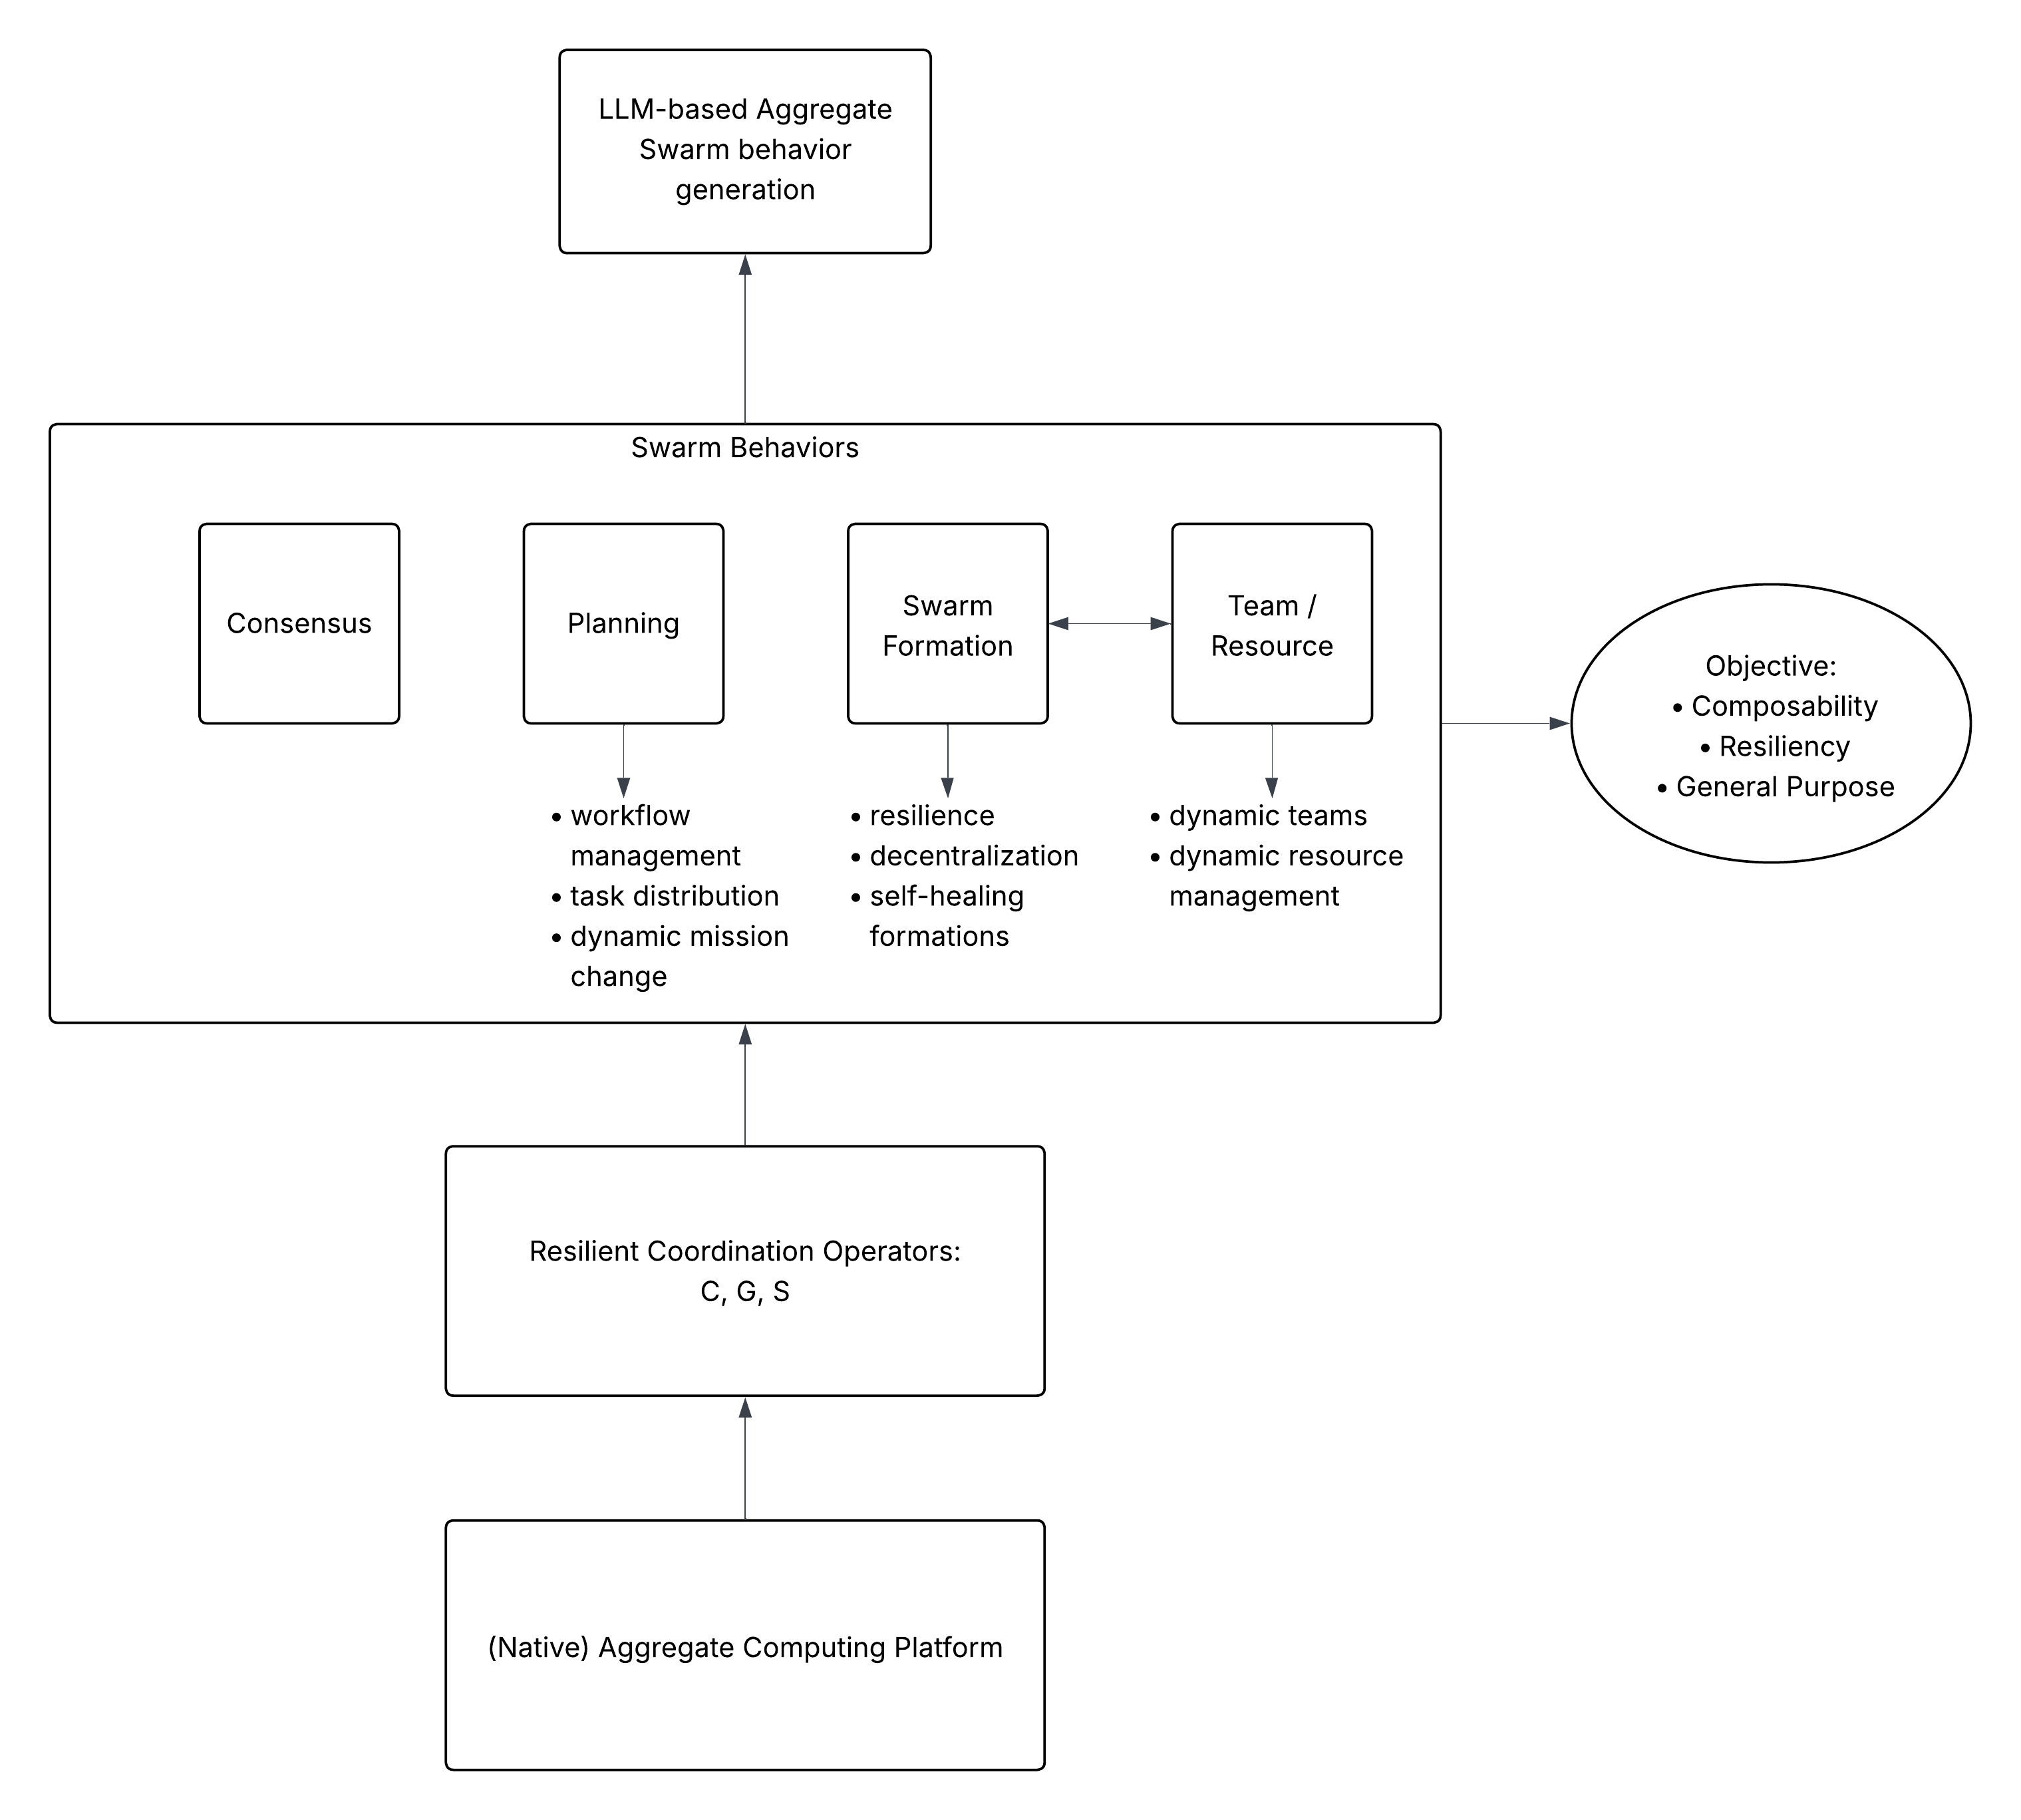
\includegraphics[width=0.7\textwidth]{figures/ResearchProject.png}
	\caption{Overview of the research project}
	 \label{fig:research-project}
\end{figure}


\subsection{Reference Scenarios}

% ----------------------------------------
\section{Expected Results}

% ----------------------------------------
\section{Lead-time for implementation}

% ----------------------------------------
\section{Proposed criteria to be used to assess the findings obtained}

\clearpage

%-----------------------------------------
\renewcommand{\refname}{References}

\bibliographystyle{plain}
\bibliography{latex}

\end{document}
